\documentclass[11pt, a4paper]{article}
\usepackage{pdfpages}
\usepackage{parallel}
\usepackage[T2A]{fontenc}
\usepackage{ucs}
\usepackage[utf8x]{inputenc}
\usepackage[polish,english,russian]{babel}
\usepackage{hyperref}
\usepackage{rotating}
\usepackage[inner=2cm,top=1.8cm,outer=2cm,bottom=2.3cm,nohead]{geometry}
\usepackage{listings}
\usepackage{graphicx}
\usepackage{wrapfig}
\usepackage{longtable}
\usepackage{indentfirst}
\usepackage{array}
\usepackage{tikzsymbols}
\usepackage{soul}
\usepackage[ruled,vlined]{algorithm2e}
%\counterwithout{figure}{section} 

\usepackage{url}
\makeatletter
\g@addto@macro{\UrlBreaks}{\UrlOrds}
\makeatother

\newcolumntype{P}[1]{>{\raggedright\arraybackslash}p{#1}}
\frenchspacing
\usepackage{fixltx2e} %text sub- and superscripts
\usepackage{icomma} % коскі ў матэматычным рэжыме
\PreloadUnicodePage{4}

\newcommand{\longpage}{\enlargethispage{\baselineskip}}
\newcommand{\shortpage}{\enlargethispage{-\baselineskip}}

\def\switchlang#1{\expandafter\csname switchlang#1\endcsname}
\def\switchlangbe{
\let\saverefname=\refname%
\def\refname{Літаратура}%
\def\figurename{Іл.}%
}
\def\switchlangen{
\let\saverefname=\refname%
\def\refname{References}%
\def\figurename{Fig.}%
}
\def\switchlangru{
\let\saverefname=\refname%
\let\savefigurename=\figurename%
\def\refname{Литература}%
\def\figurename{Рис.}%
}

\hyphenation{admi-ni-stra-tive}
\hyphenation{ex-pe-ri-ence}
\hyphenation{fle-xi-bi-li-ty}
\hyphenation{Py-thon}
\hyphenation{ma-the-ma-ti-cal}
\hyphenation{re-ported}
\hyphenation{imp-le-menta-tions}
\hyphenation{pro-vides}
\hyphenation{en-gi-neering}
\hyphenation{com-pa-ti-bi-li-ty}
\hyphenation{im-pos-sible}
\hyphenation{desk-top}
\hyphenation{elec-tro-nic}
\hyphenation{com-pa-ny}
\hyphenation{de-ve-lop-ment}
\hyphenation{de-ve-loping}
\hyphenation{de-ve-lop}
\hyphenation{da-ta-ba-se}
\hyphenation{plat-forms}
\hyphenation{or-ga-ni-za-tion}
\hyphenation{pro-gramming}
\hyphenation{in-stru-ments}
\hyphenation{Li-nux}
\hyphenation{sour-ce}
\hyphenation{en-vi-ron-ment}
\hyphenation{Te-le-pathy}
\hyphenation{Li-nux-ov-ka}
\hyphenation{Open-BSD}
\hyphenation{Free-BSD}
\hyphenation{men-ti-on-ed}
\hyphenation{app-li-ca-tion}

\def\progref!#1!{\texttt{#1}}
\renewcommand{\arraystretch}{2} %Іначай формулы ў матрыцы зліпаюцца з лініямі
\usepackage{array}

\def\interview #1 (#2), #3, #4, #5\par{

\section[#1, #3, #4]{#1 -- #3, #4}
\def\qname{LVEE}
\def\aname{#1}
\def\q ##1\par{{\noindent \bf \qname: ##1 }\par}
\def\a{{\noindent \bf \aname: } \def\qname{L}\def\aname{#2}}
}

\def\interview* #1 (#2), #3, #4, #5\par{

\section*{#1\\{\small\rm #3, #4. #5}}
\ifx\ParallelWhichBox\undefined%
    \addcontentsline{toc}{section}{#1, #3, #4}%
\else%
\ifnum\ParallelWhichBox=0%
    \addcontentsline{toc}{section}{#1, #3, #4}%
\fi\fi%

\def\qname{LVEE}
\def\aname{#1}
\def\q ##1\par{{\noindent \bf \qname: ##1 }\par}
\def\a{{\noindent \bf \aname: } \def\qname{L}\def\aname{#2}}
}

\newcommand{\interviewfooter}[1]{
\vskip 1em
\noindent \textit{#1}
}

\switchlang{en}
\begin{document}

\title{2000 "--- IBM ScrollPoint II mouse}
\date{}
\maketitle
\selectlanguage{english}
The MO09K model, released around 2000, was the second generation of the IBM ScrollPoint mouse that debuted in 1998 \cite{hist}. A feature of this IBM mouse was the replacement of the scroll wheel with the trackpoint -- a miniature analog stick (actually, a strain gauge joystick), similar to the cursor controls used in the ThinkPad line of laptops. Trackpoint integration made the IBM ScrollPoint the first mouse to support both horizontal and vertical scrolling \cite{buxtonG1}. In this case, the direction of scrolling is determined by the direction of pressing the joystick, and its speed is set by the pressing force.

\begin{figure}[h]
    \centering
    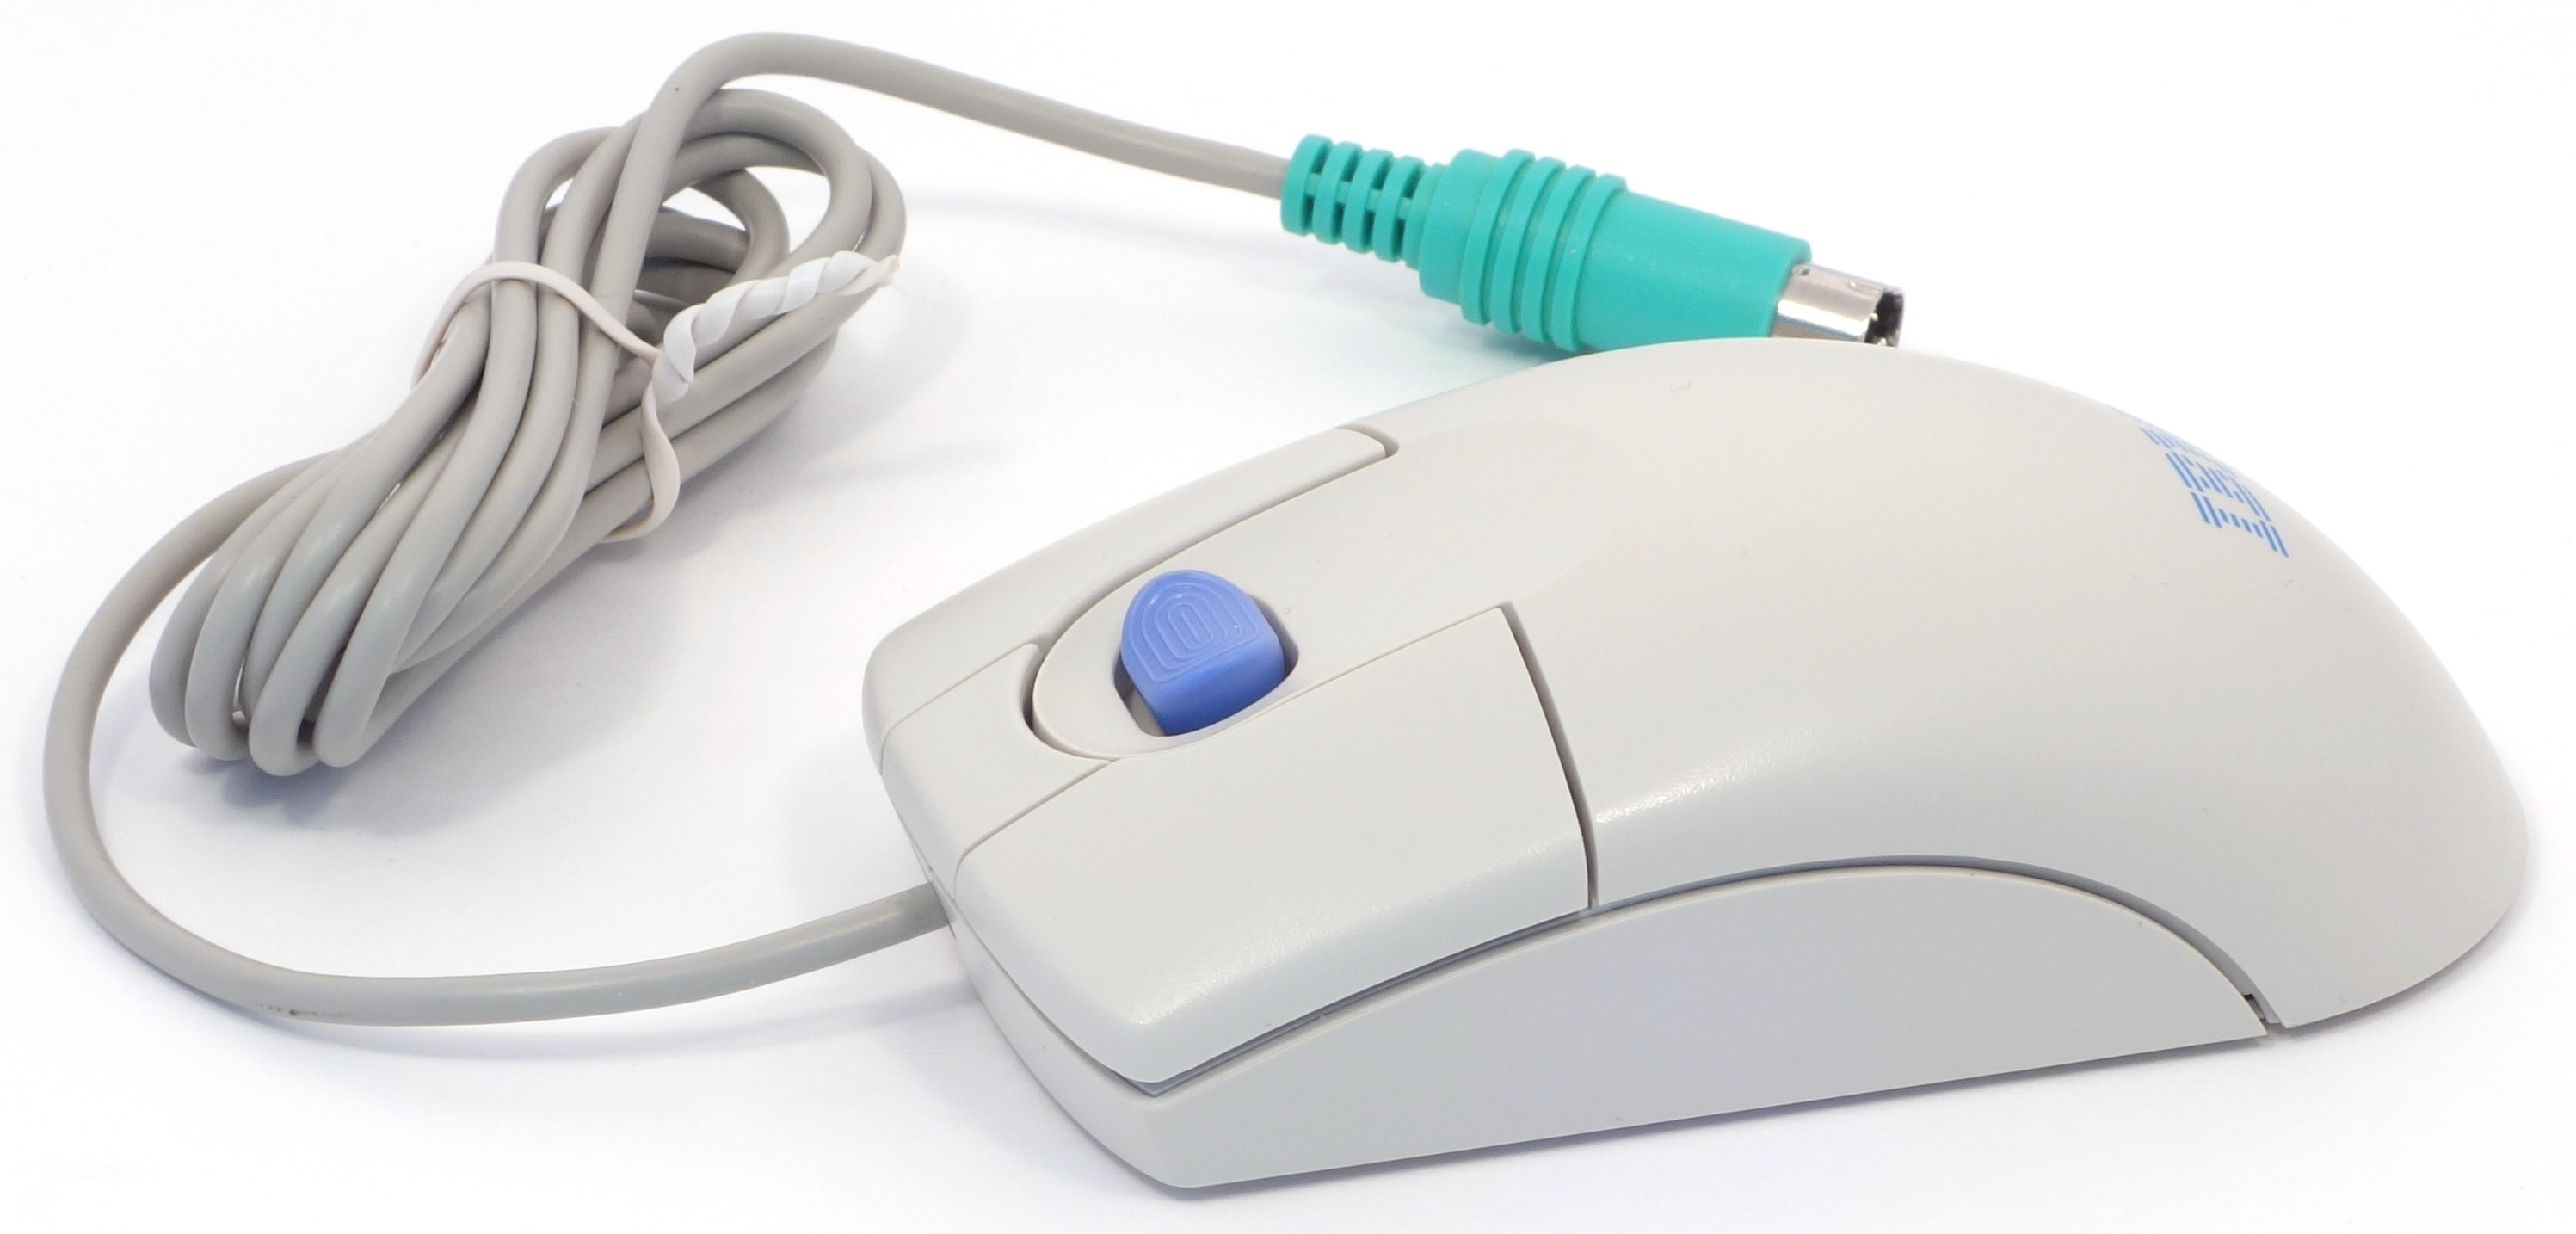
\includegraphics[scale=0.65]{2000_ibm_scrollpoint_ii_mouse/pic_30.jpg}
    \caption{IBM ScrollPoint II mouse}
    \label{fig:IBMScrollPointIIPic}
\end{figure}

The second generation of the ScrollPoint mouse received a slightly more rounded body, a new shape of the rubber joystick tip, and a third button located directly after it (fig. \ref{fig:IBMScrollPointIITopBottom}).

\begin{figure}[h]
    \centering
    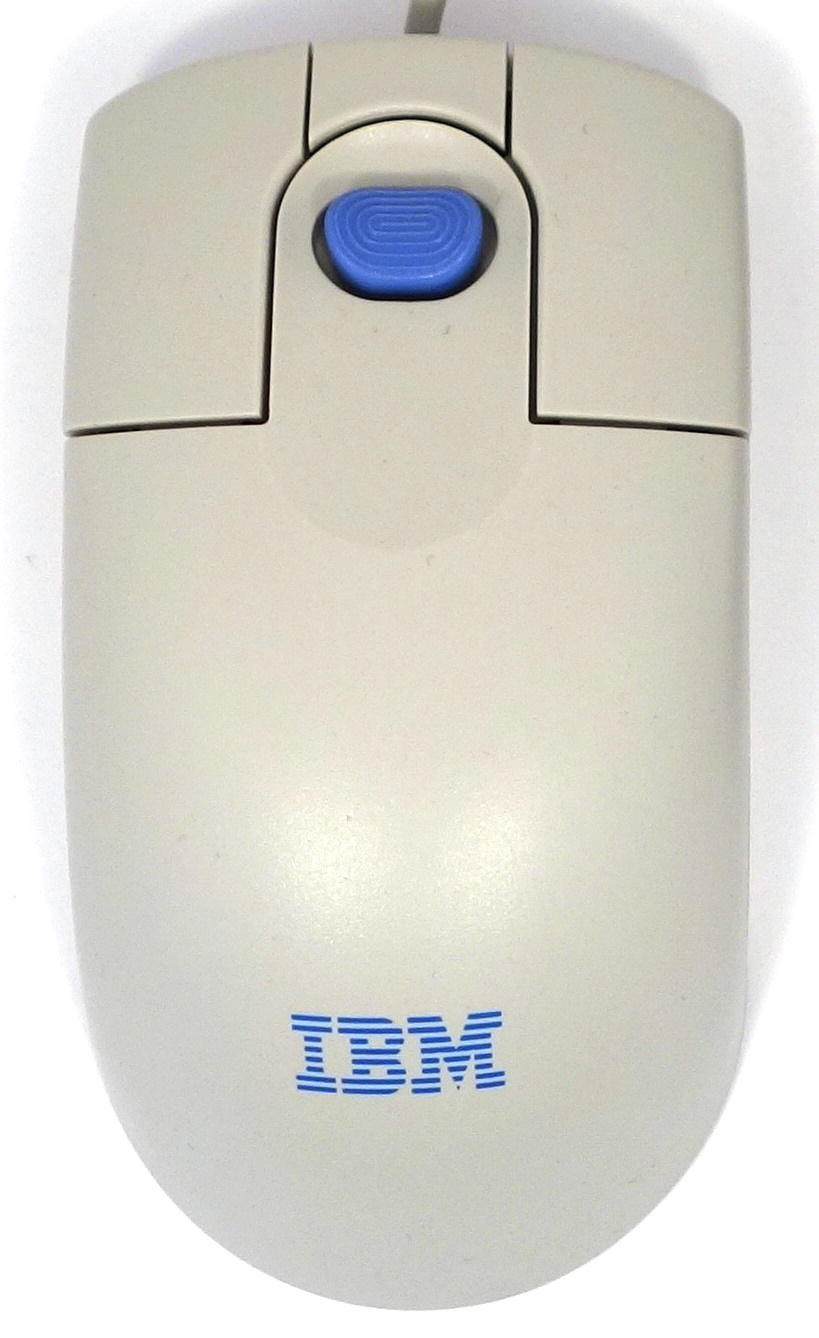
\includegraphics[scale=0.75]{2000_ibm_scrollpoint_ii_mouse/top_30.jpg}
    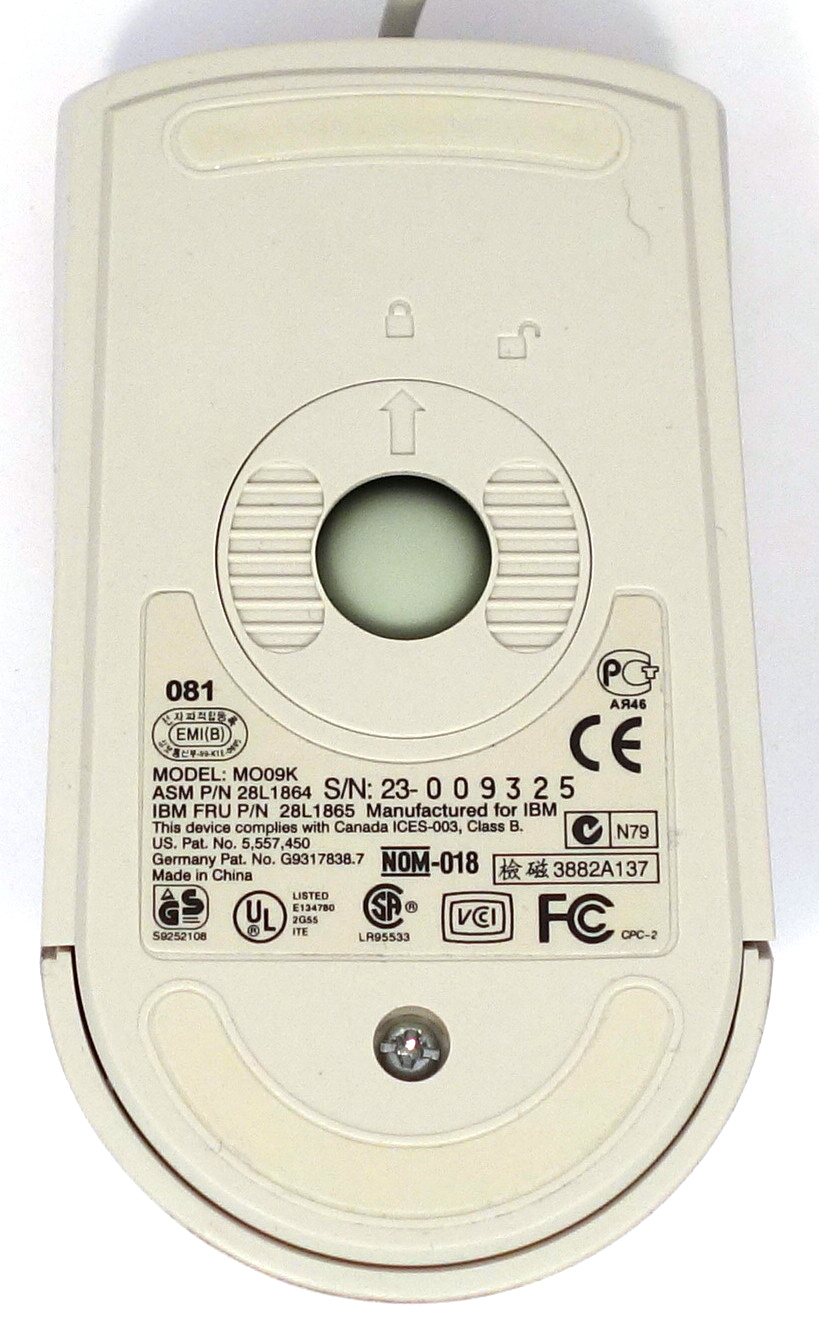
\includegraphics[scale=0.75]{2000_ibm_scrollpoint_ii_mouse/bottom_30.jpg}
    \caption{IBM ScrollPoint II mouse, top and bottom views}
    \label{fig:IBMScrollPointIITopBottom}
\end{figure}

Replacing the traditional round tip of the trackpoint with a kind of concave ribbed rocker was intended to facilitate horizontal scrolling. It is known that the fingers are less adapted to applying force sideways than downwards. Pressing vertically with the middle finger near the edge of the concave surface should, through a lever effect, facilitate horizontal scrolling \cite{buxtonG2}.

\begin{figure}[h]
    \centering
    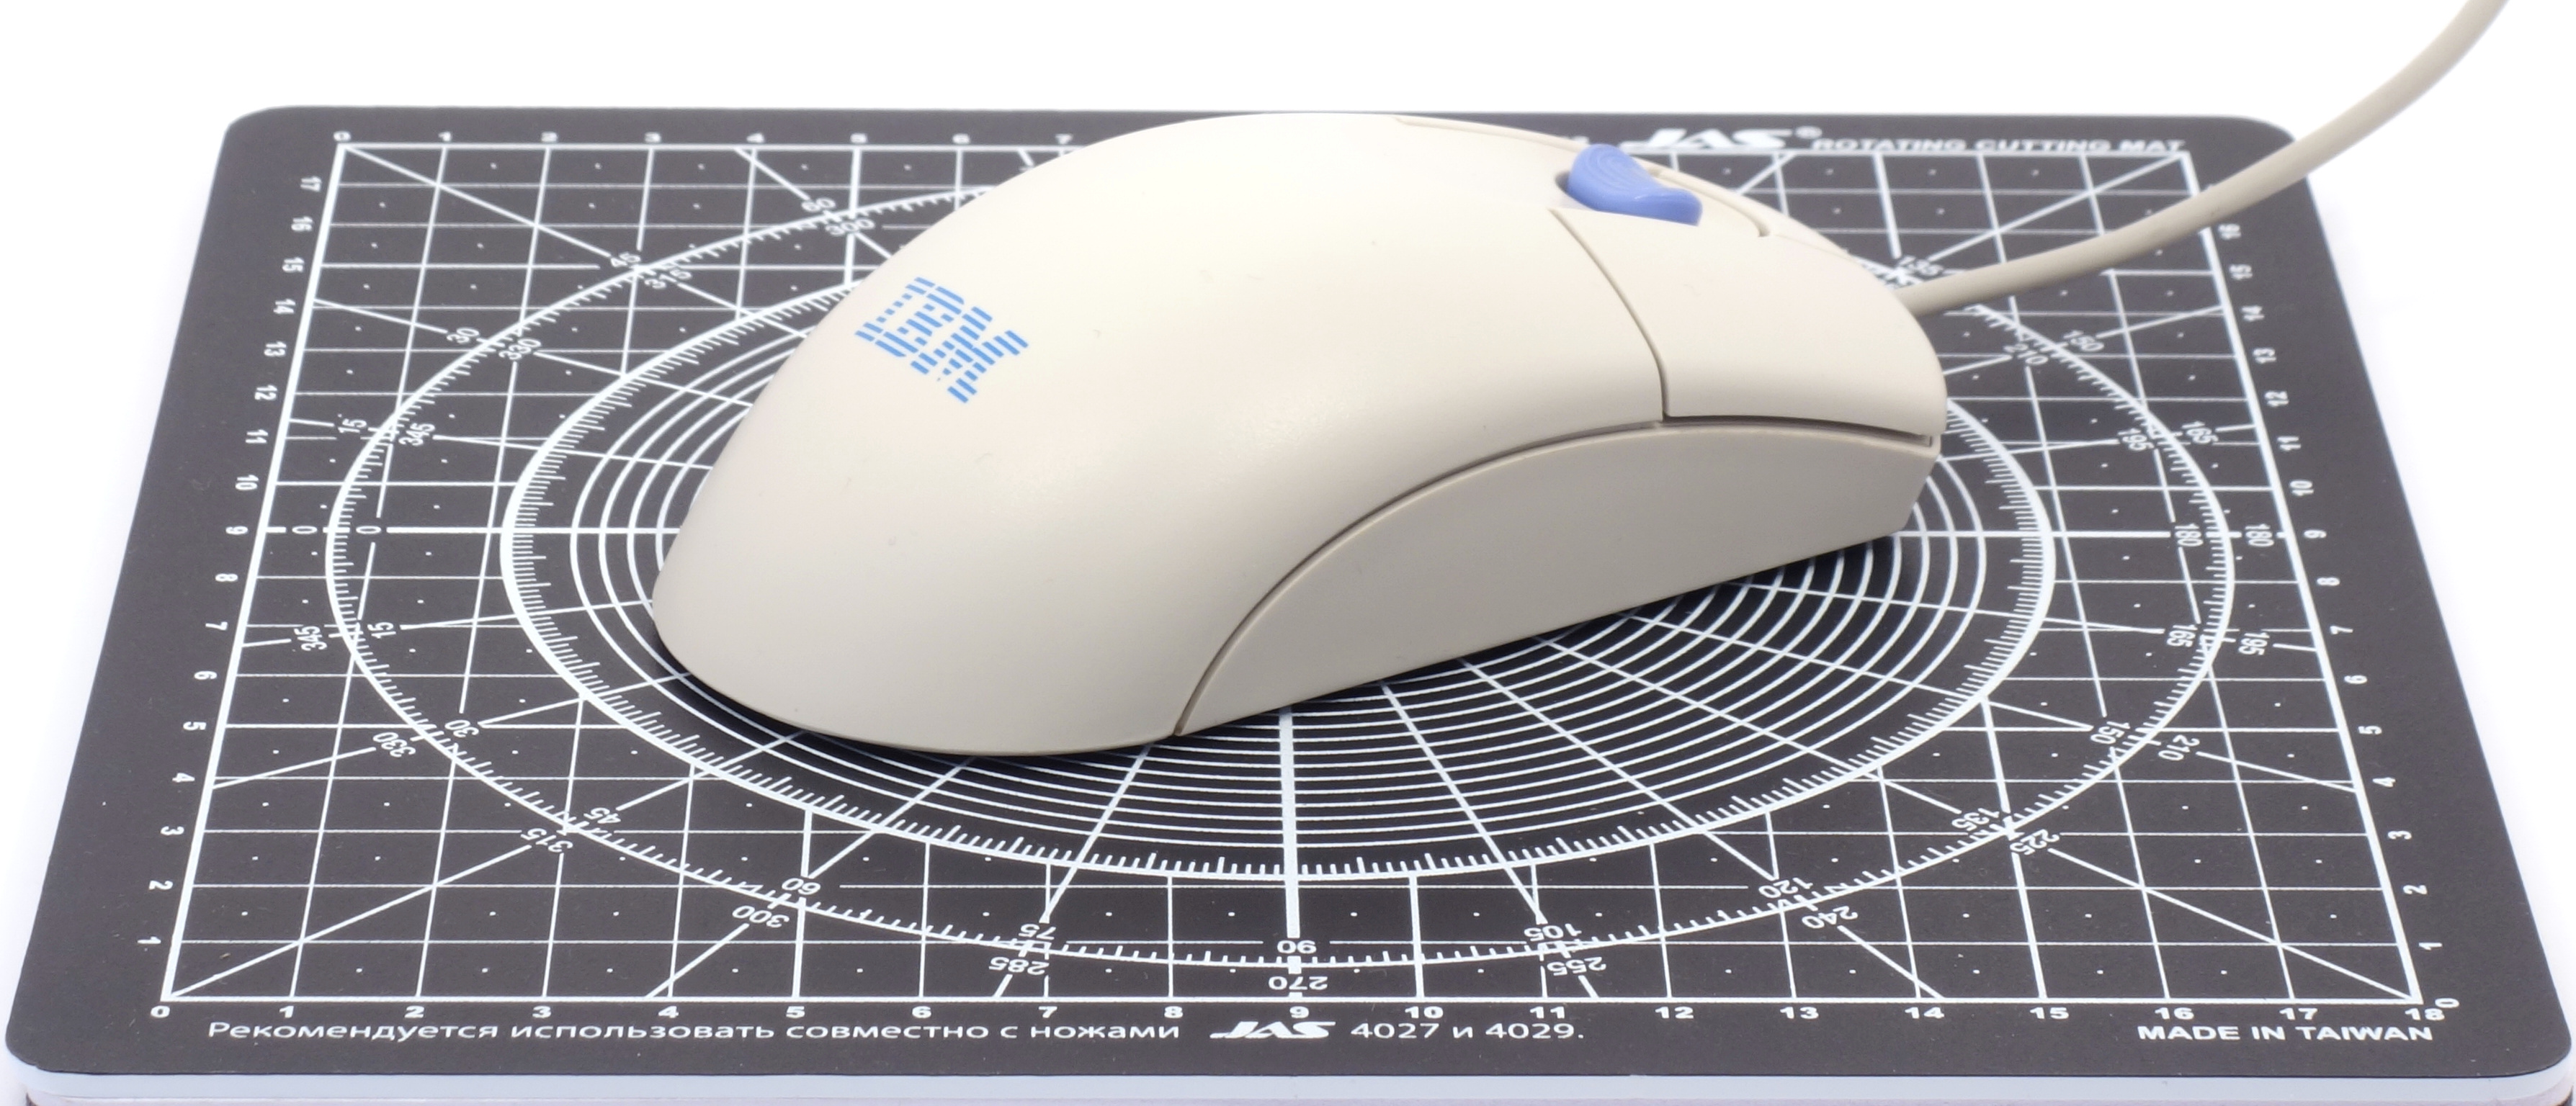
\includegraphics[scale=0.54]{2000_ibm_scrollpoint_ii_mouse/size_30.jpg}
    \caption{IBM ScrollPoint II mouse on a graduated pad with a grid step of 1~cm}
    \label{fig:IBMPS2Size}
\end{figure}

As can be seen in fig. (Fig. \ref{fig:IBMPS2Size}), the mouse is medium in size. The curved shape of the case allows the user to comfortably lean on it with the palm \ref{fig:IBMScrollPointIIHand} and press the buttons with a fairly natural position of the hand. At the same time, the case is symmetrical and equally suitable for left-handers and right-handers.


\begin{figure}[h]
    \centering
    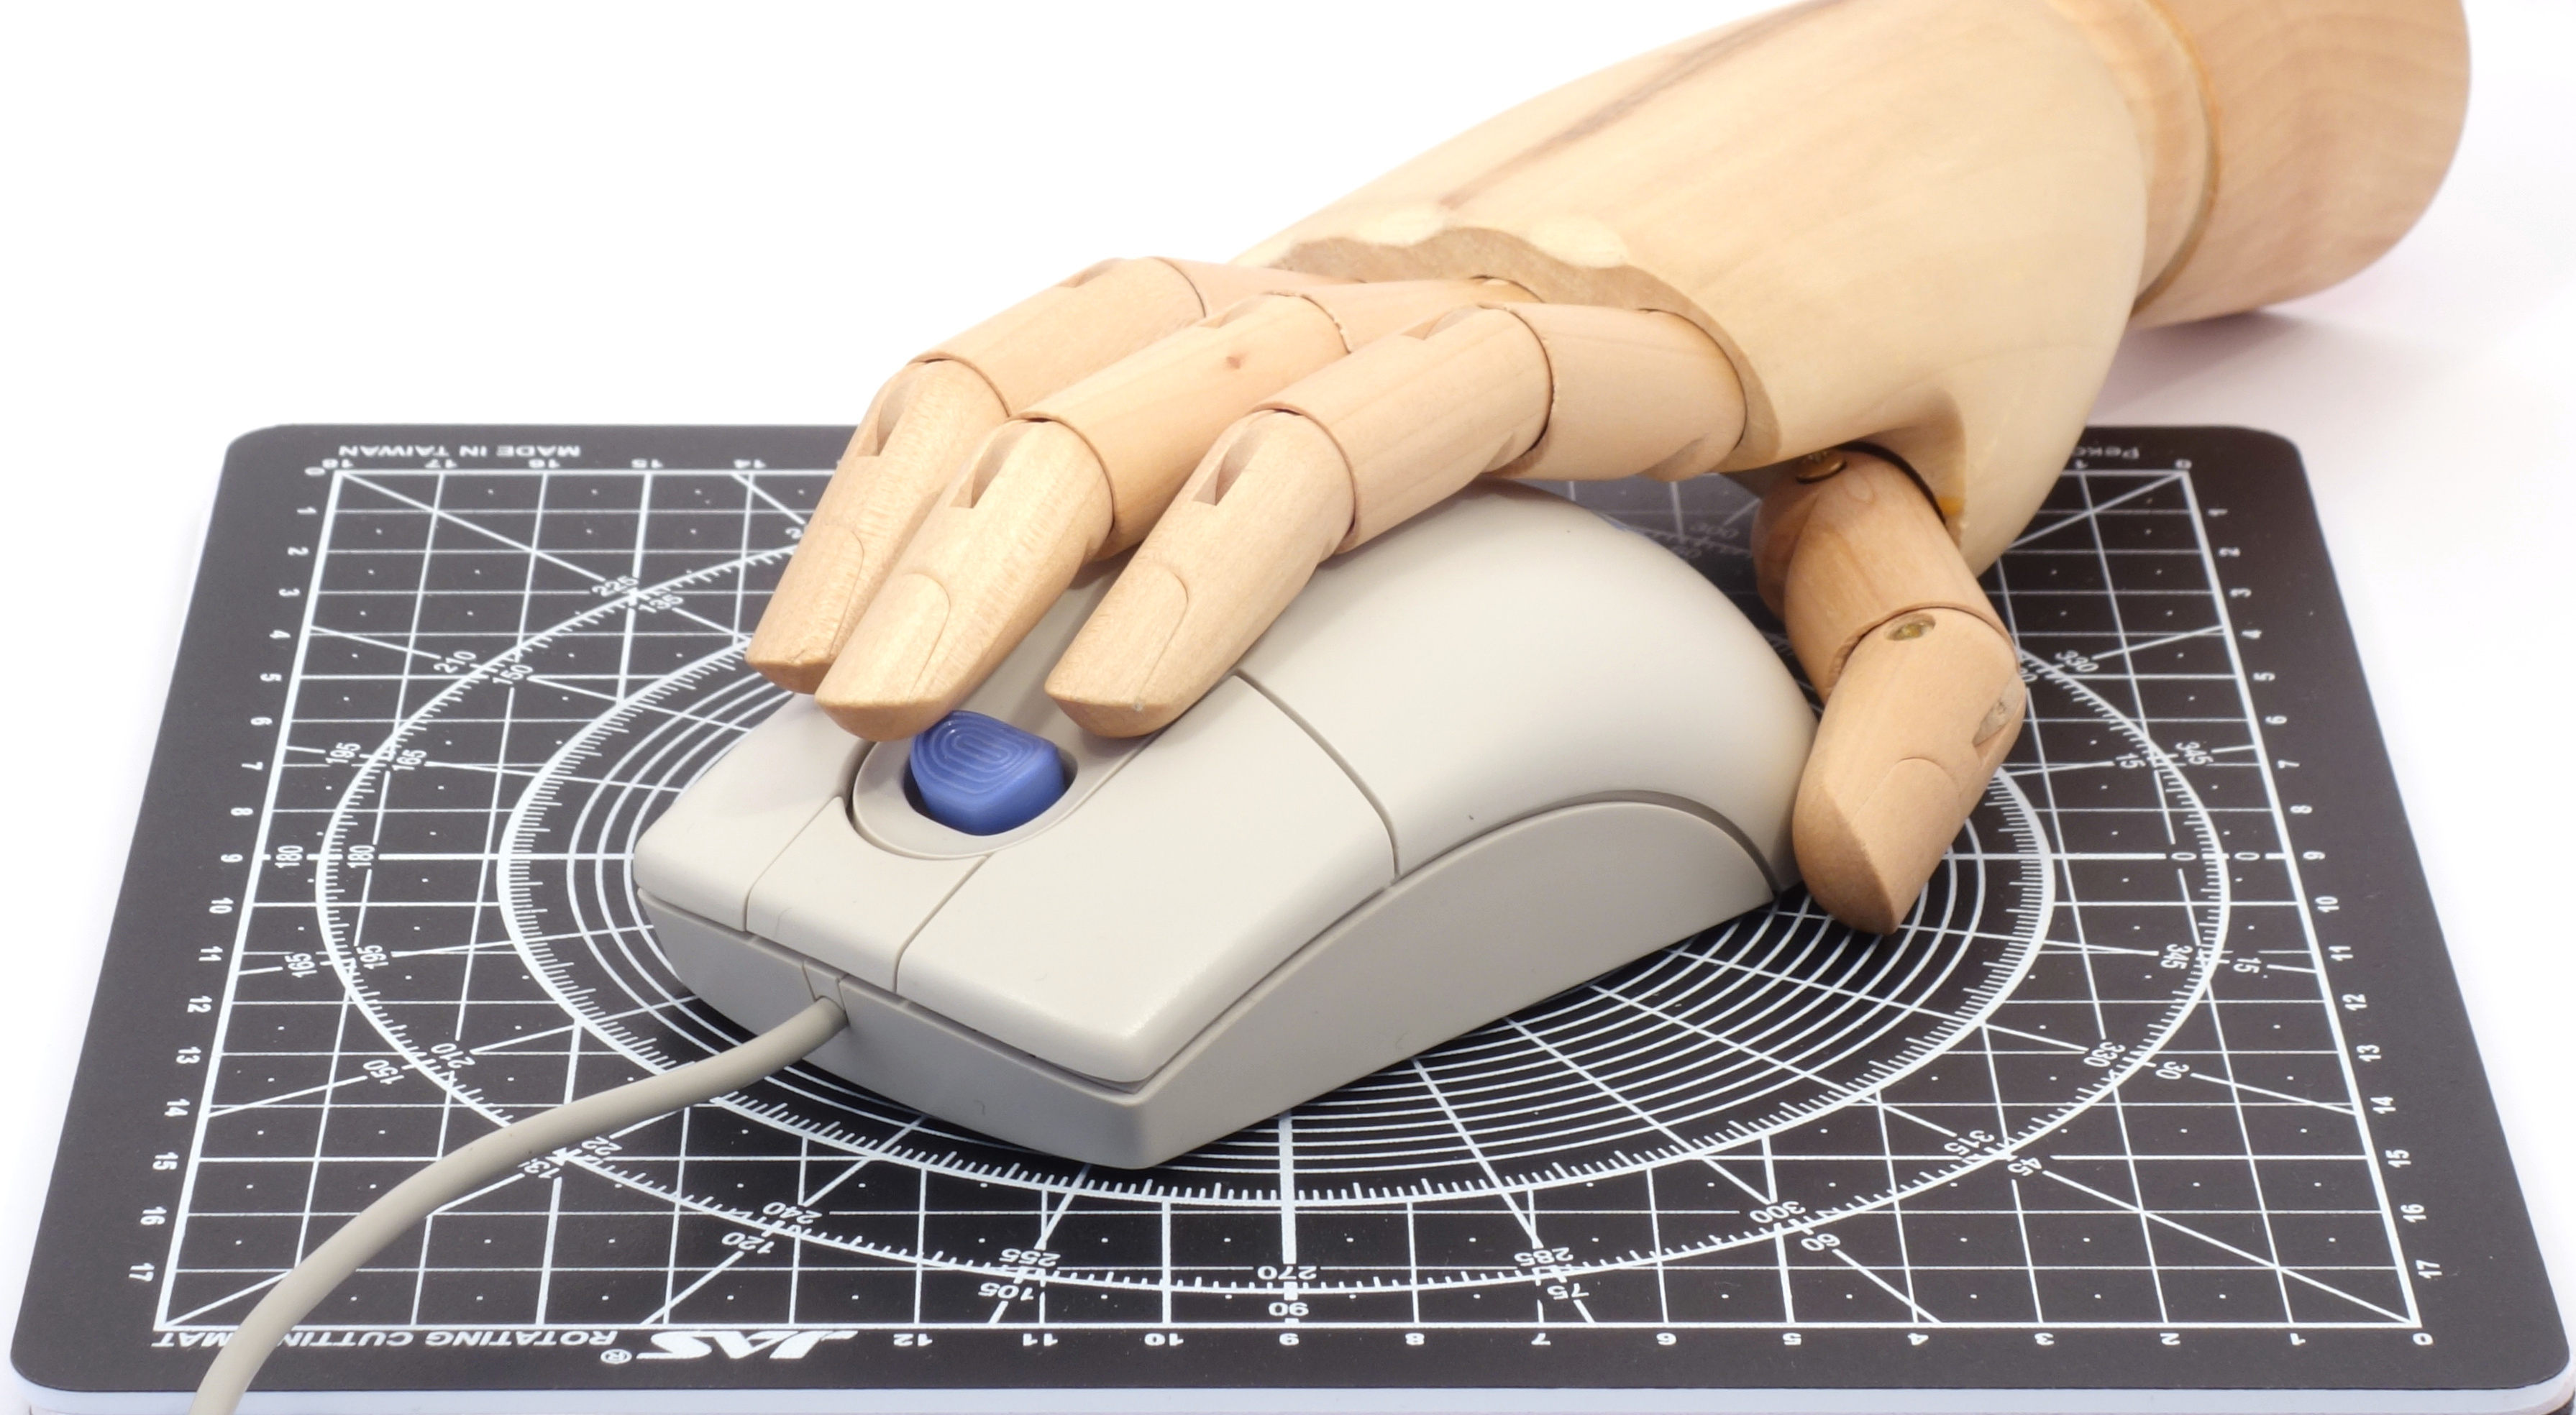
\includegraphics[scale=0.6]{2000_ibm_scrollpoint_ii_mouse/hand_30.jpg}
    \caption{IBM ScrollPoint II mouse with a human hand model}
    \label{fig:IBMScrollPointIIHand}
\end{figure}

The internals of the IBM ScrollPoint II mouse are shown in fig. \ref{fig:IBMPS2Inside}, which makes it possible to classify the mouse as a typical (besides the pointing stick) device with an optomechanical encoder. However, the design of the mouse shows clear signs of conservatism: a typical example is the plastic protection shell of the ball, typical for mice produced in the first half of the nineties, but not in 2000s.

\begin{figure}[h]
    \centering
    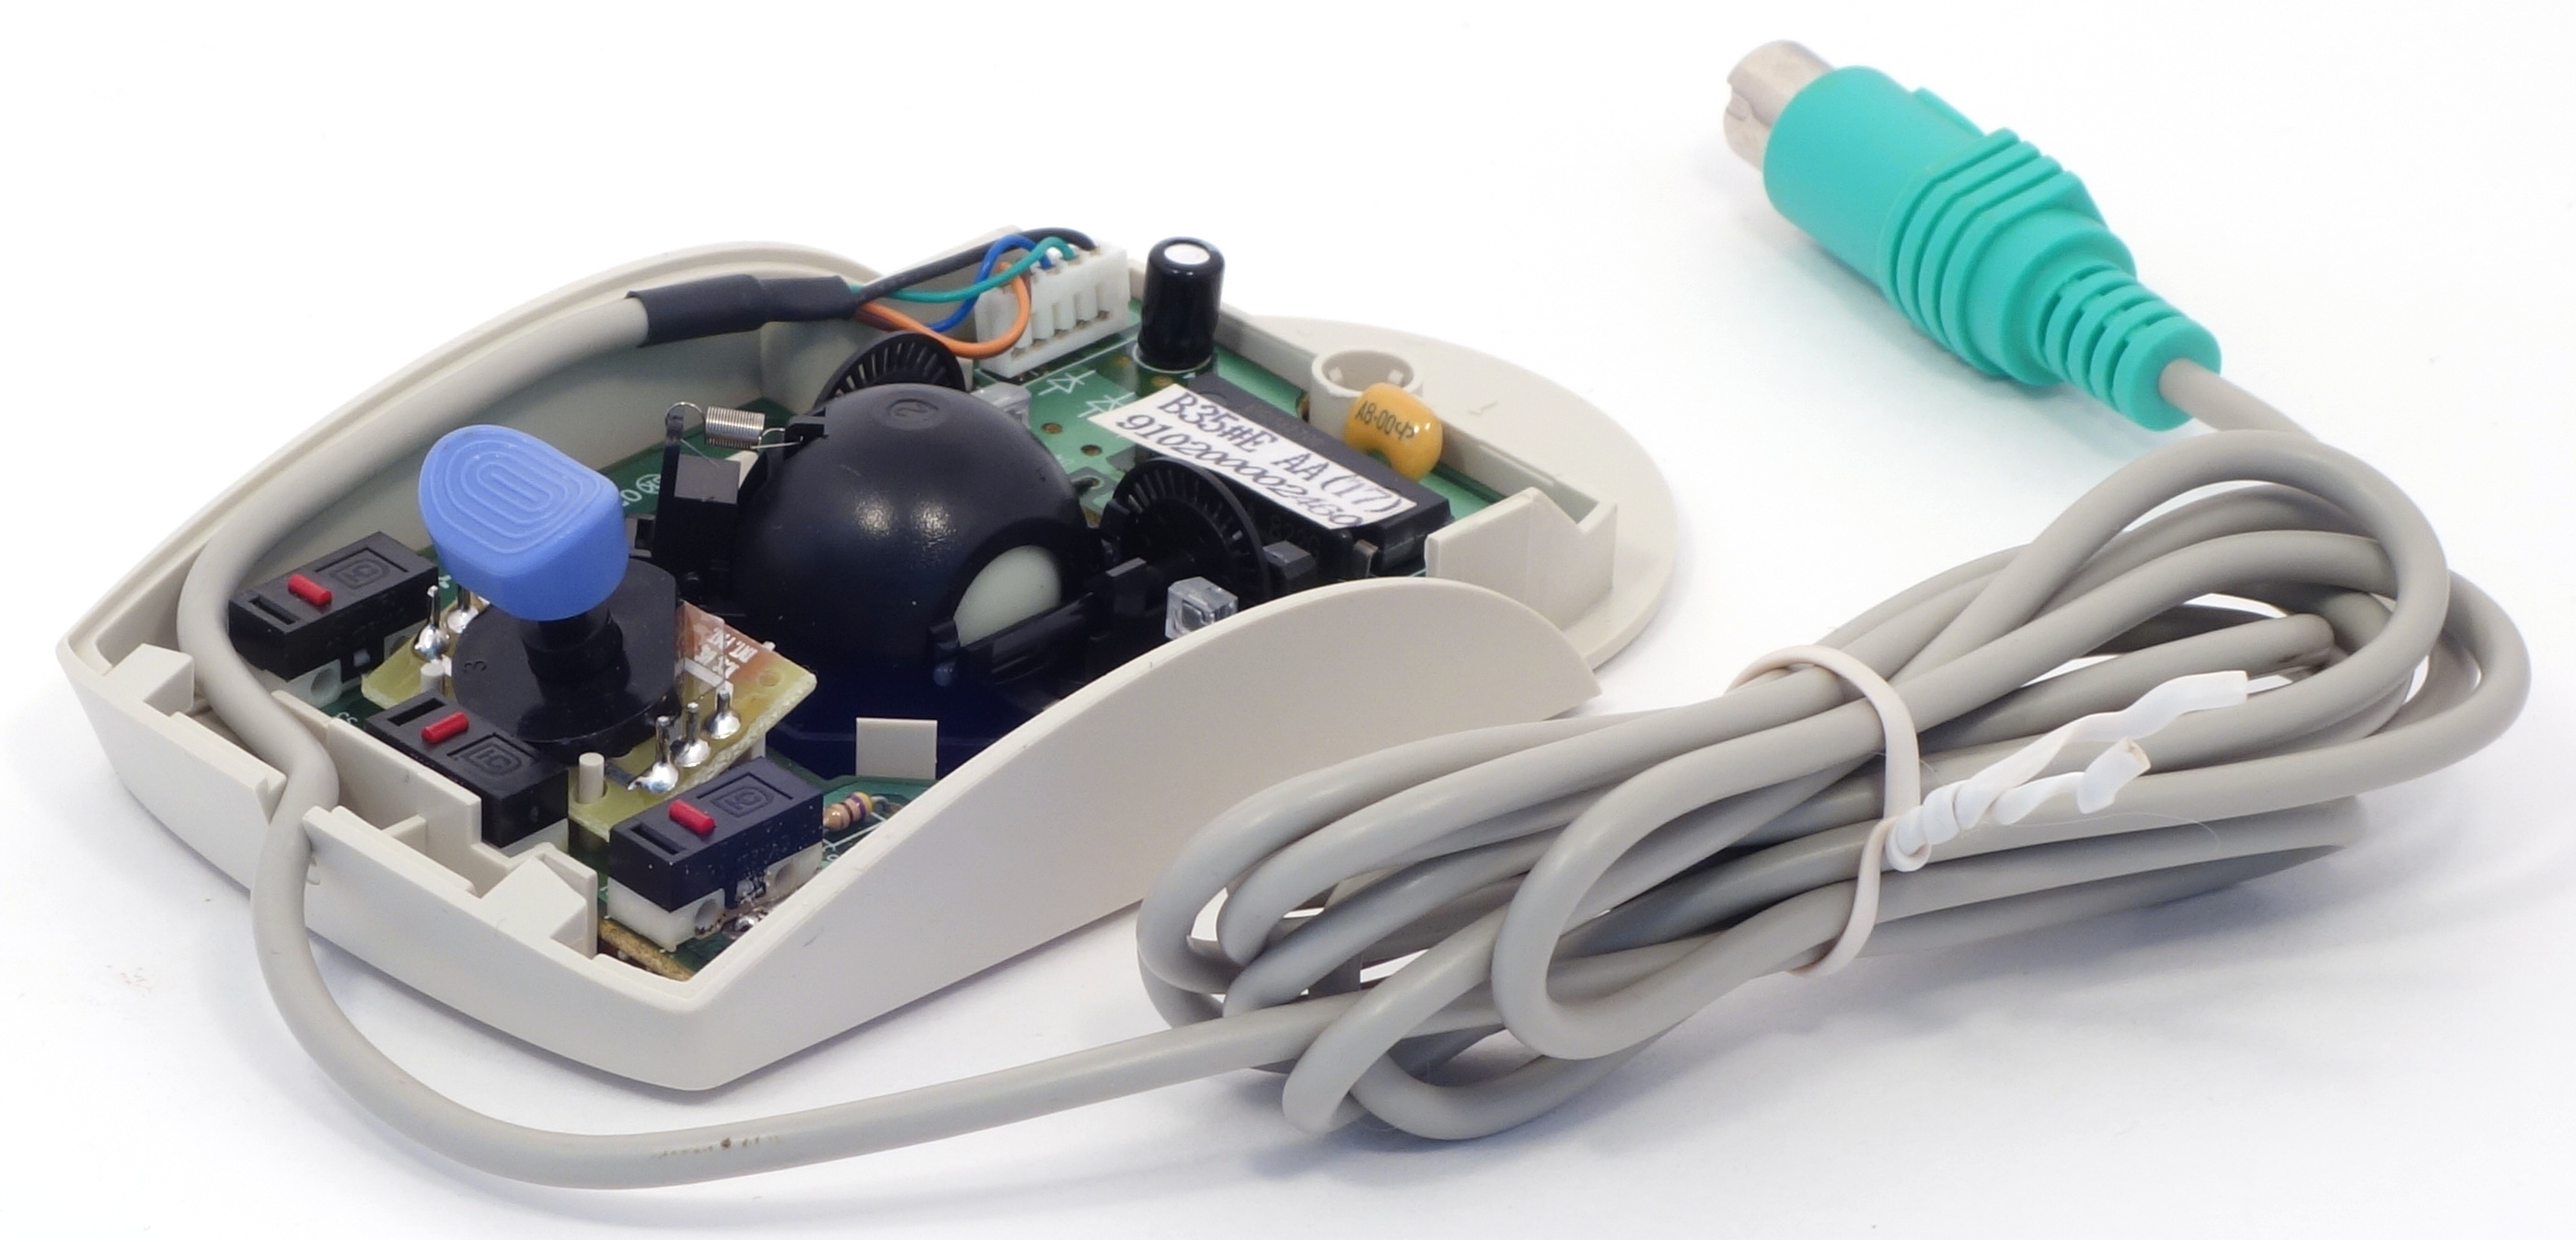
\includegraphics[scale=0.7]{2000_ibm_scrollpoint_ii_mouse/inside_30.jpg} 
    \caption{IBM ScrollPoint II mouse disassembled}
    \label{fig:IBMPS2Inside}
\end{figure}

\begin{thebibliography}{9}
    \bibitem {buxtonG1} Bill Buxton. TrackPoint Mouse G1 -- Buxton Collection. \url{https://www.microsoft.com/buxtoncollection/detail.aspx?id=120}
    \bibitem {buxtonG2} Bill Buxton. TrackPoint Mouse G2 -- Buxton Collection. \url{https://www.microsoft.com/buxtoncollection/detail.aspx?id=121}
    \bibitem {hist} IBM ScrollPoint Information and Software -- ibmfiles.com // \url{http://www.ibmfiles.com/pages/scrollpoint.htm}
\end{thebibliography}

\end{document}
